\section{Auswertung und Diskussion}
\label{sec:Auswertung}

\subsection*{Bestrahlungsplan für das PTV1}

Die sich bei dem ersten Bestrahlungsplan ergebende Dosisverteilung ist aus verschiedenen
Ansichten in den Abbildungen \ref{abb:Z1}, \ref{abb:Y1} und \ref{abb:X1} dargestellt.
Anhand der Dosisverteilung ist zu erkennen, dass das PTV1 nicht komplett mit der $95\%$
Isodosenlinie umschlossen werden konnte. Vor allem in den Bereich des PTVs, der sehr nah an
die Lunge heranreicht ist nicht die gewünschte Dosis appliziert worden. Das kommt daher, da die
Lunge ein Risikoorgan ist und deshalb geschont werden muss. Die maximale relative Dosis
bei dieser Bestrahlung ist $108,9\%$ und wird in dem PTV appliziert. Diese maximale Dosis
liegt etwas oberhalb der vorgeschriebenen maximalen Dosis von $107\%$ \cite{ICRU}.
Da diese Dosis allerdings in dem PTV appliziert wird und sie nur knapp oberhalb der erlaubten maximalen
Dosis liegt, ist die maximale relative Dosis akzeptabel. Die minimale relative Dosis in dem PTV liegt bei
$83,8\%$ und liegt etwas unterhalb der gewünschten Dosis von $95\%$.

\begin{figure}[H]
  \centering
  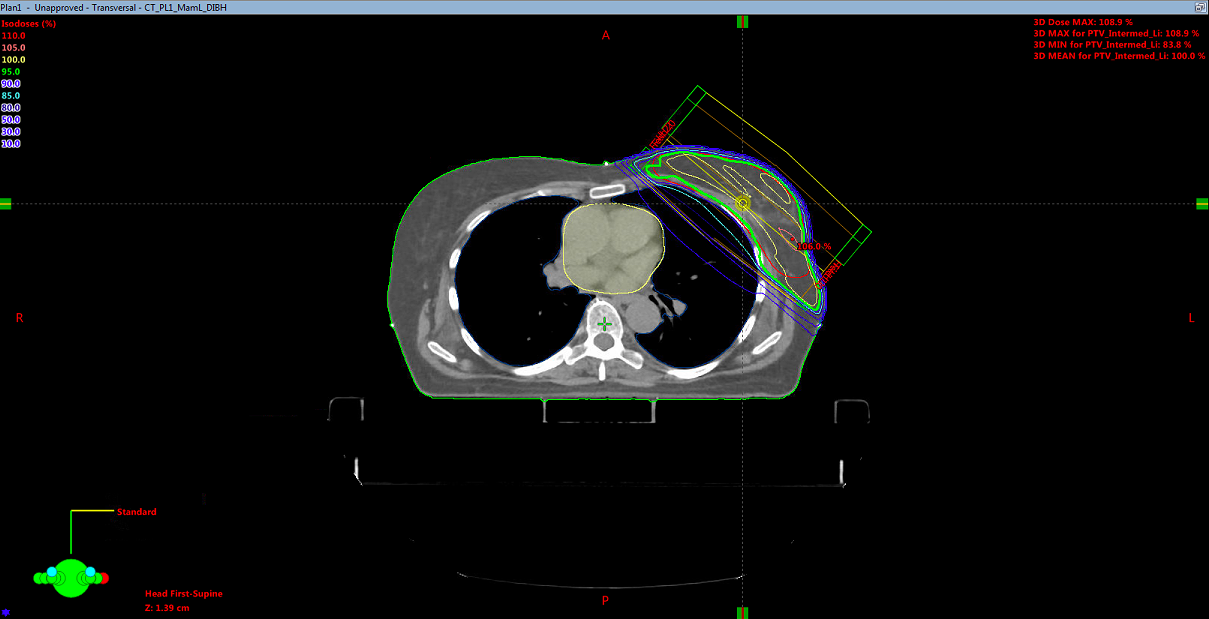
\includegraphics[width=\textwidth]{Bilder/Mamma1_Z.png}
  \caption{Darstellung der Dosisverteilung im Thorax in Transversalansicht.}
  \label{abb:Z1}
\end{figure}

\begin{figure}[H]
  \centering
  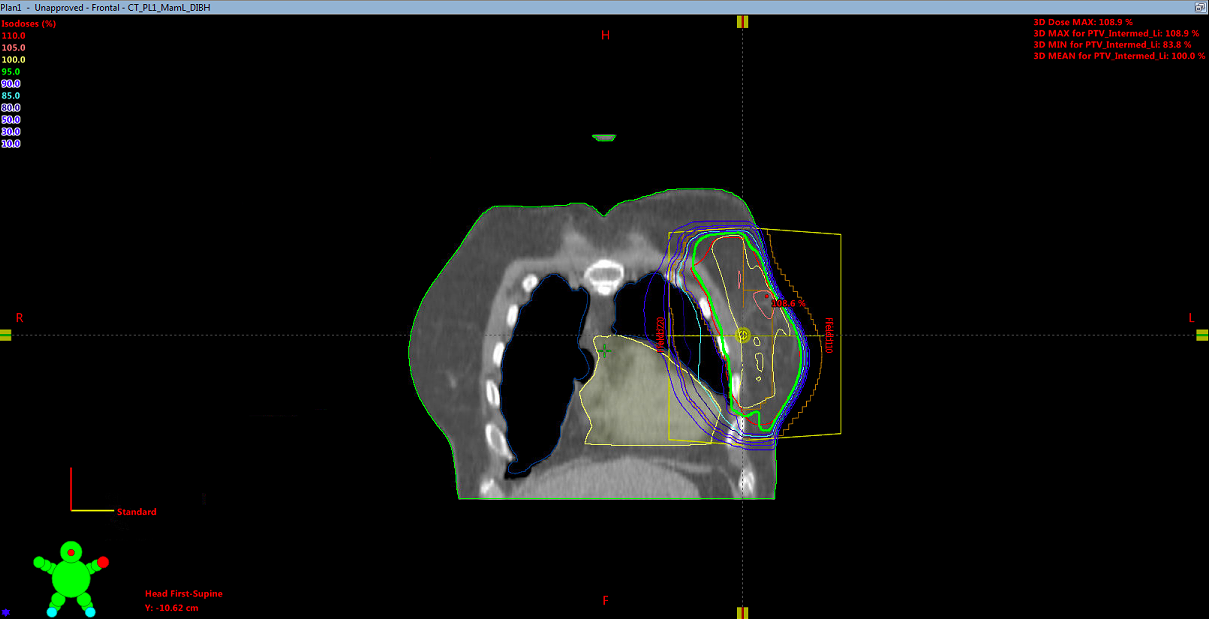
\includegraphics[width=\textwidth]{Bilder/Mamma1_Y.png}
  \caption{Darstellung der Dosisverteilung im Thorax in Frontalansicht.}
  \label{abb:Y1}
\end{figure}

\begin{figure}[H]
  \centering
  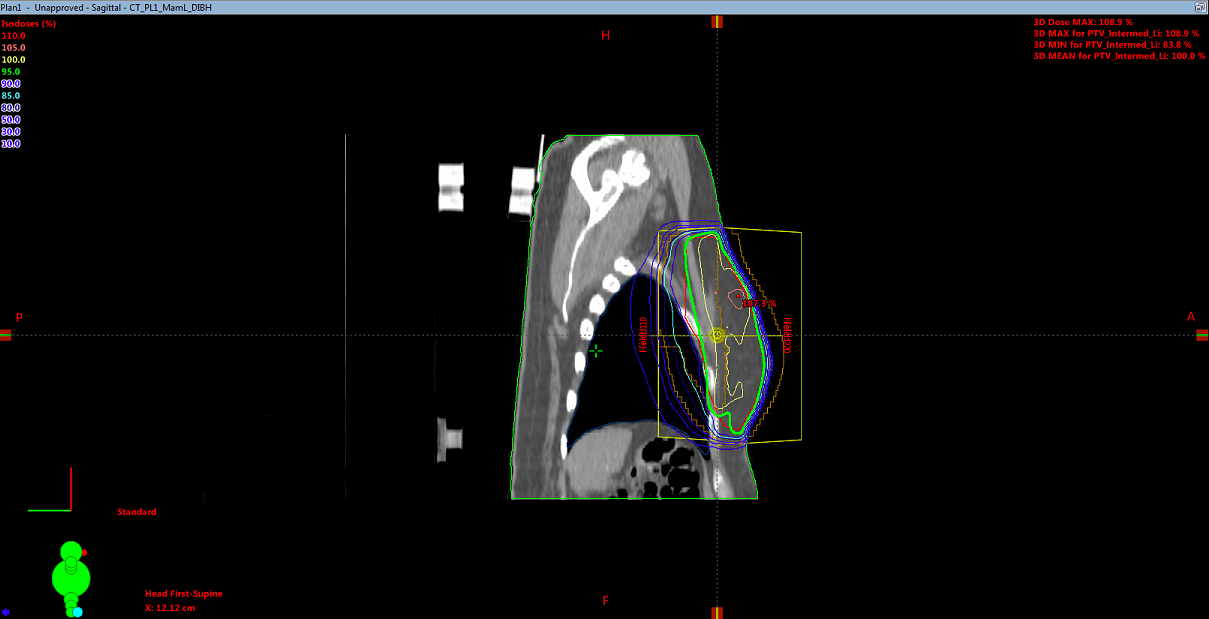
\includegraphics[width=\textwidth]{Bilder/Mamma1_X.png}
  \caption{Darstellung der Dosisverteilung im Thorax in Sagittalansicht.}
  \label{abb:X1}
\end{figure}


Um die Dosisverteilung besser beurteilen zu können ist in der Abbildung \ref{abb:DVH}
das DVH dieses Bestrahlungsplanes gezeigt. Anhand der DVH Kurve für das PTV1 (rot) ist
zu erkennen, dass $93\%$ des PTVs noch eine relative Dosis von $95\%$ erhält. Das bedeutet,
dass nur ein kleiner Teil des PTVs nicht mit der $95\%$ Isodosenlinie umschlossen werden konnte.
Anhand der DVH Kurve des gesamten Thorax (grün) ist gut zu erkennen, dass in dem Großteil des Volumens
nur eine geringe Dosis appliziert wird. In etwa $7\%$ des Volumens wird noch eine
relative Dosis von $50\%$ appliziert. Es ist auch zu erkennen, dass die rechte Mamma nur eine sehr geringe
Dosis erhält. Auch die Risikoorgane, das Herz und die Lunge, werden bei diesen Bestrahlungsplan
geschont. In der gesamten Lunge wird in weniger als $10\%$ des Volumens noch eine relative Dosis von $50\%$
appliziert. In dem Herzen wird in etwa $9\%$ des Volumens eine relative Dosis von $20\%$ appliziert.
Die Einhaltung der Organdosisgrenzwerte wird am Ende anhand der Summe der beiden Bestrahlungspläne überprüft.

\begin{figure}[H]
  \centering
  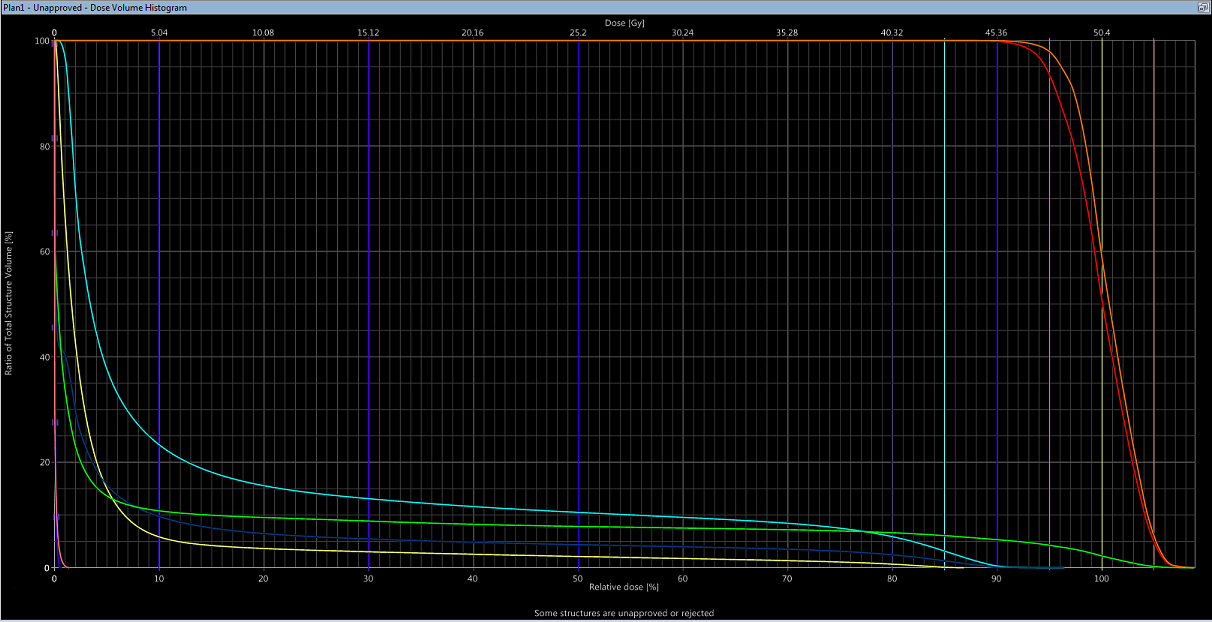
\includegraphics[width=\textwidth]{Bilder/DVH1.png}
  \caption{Dosis-Volumen-Histogramm für das PTV1 in rot und den gesamten Thorax in grün. Außerdem ist das DVH für das Herz in gelb, für die linke Lunge in hellblau, für die rechte Lunge in blau, für die gesamte Lunge in dunkelblau, für die rechte Mamma in pink und für das CTV1 in braun dargestellt.}
  \label{abb:DVH}
\end{figure}

\subsection*{Bestrahlungsplan für das PTV2}

Die Dosisverteilung der zweiten Bestrahlungsplans ist aus verschiedenen Ansichten in
den Abbildungen \ref{abb:Z2}, \ref{abb:Y2} und \ref{abb:X2} gezeigt. Dabei ist zu erkennen,
dass das PTV2 gut mit der $95\%$ Isodosenlinie umschlossen werden konnte. Die
minimale relative Dosis in dem PTV2 ist $88,6\%$, was bedeutet, dass das PTV nicht komplett von
der $95\%$ Isodosenlinie umschlossen wurde. Allerdings ist es nur ein sehr kleiner
Teil des PTVs, das nicht umschlossen werden konnte. Die maximale relative Dosis liegt bei
$104,2\%$ und wird in dem PTV2 appliziert. Diese Dosis liegt unterhalb der erlaubten maximalen
Dosis.

\begin{figure}[H]
  \centering
  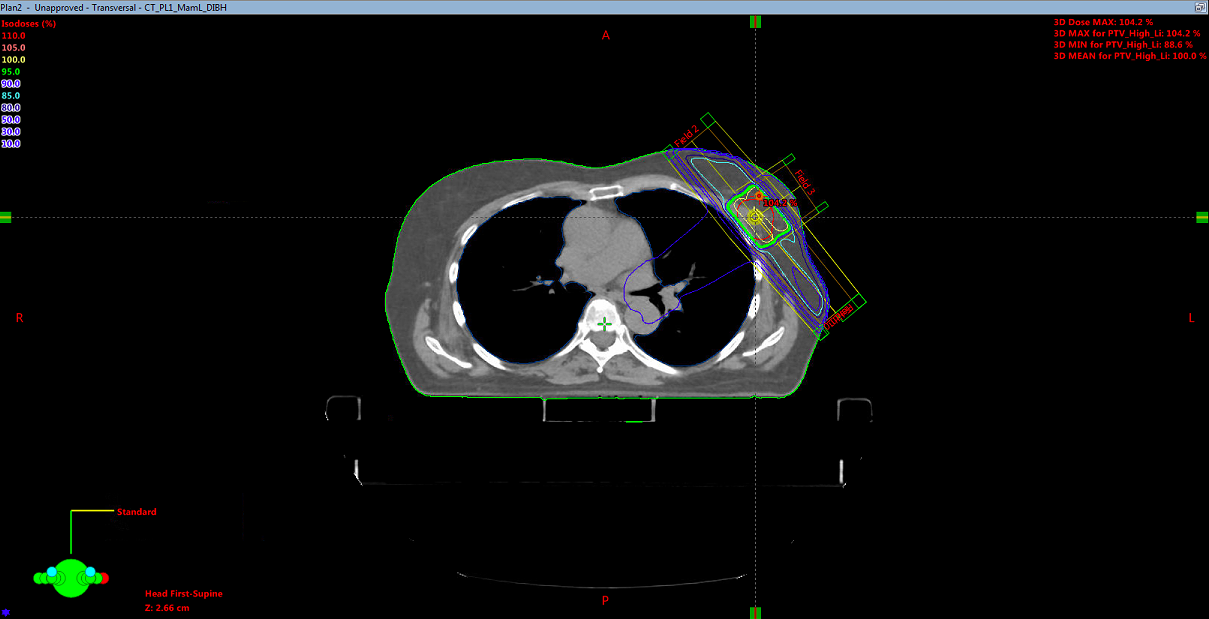
\includegraphics[width=\textwidth]{Bilder/Mamma2_Z.png}
  \caption{Darstellung der Dosisverteilung im Thorax in Transversalansicht.}
  \label{abb:Z2}
\end{figure}

\begin{figure}[H]
  \centering
  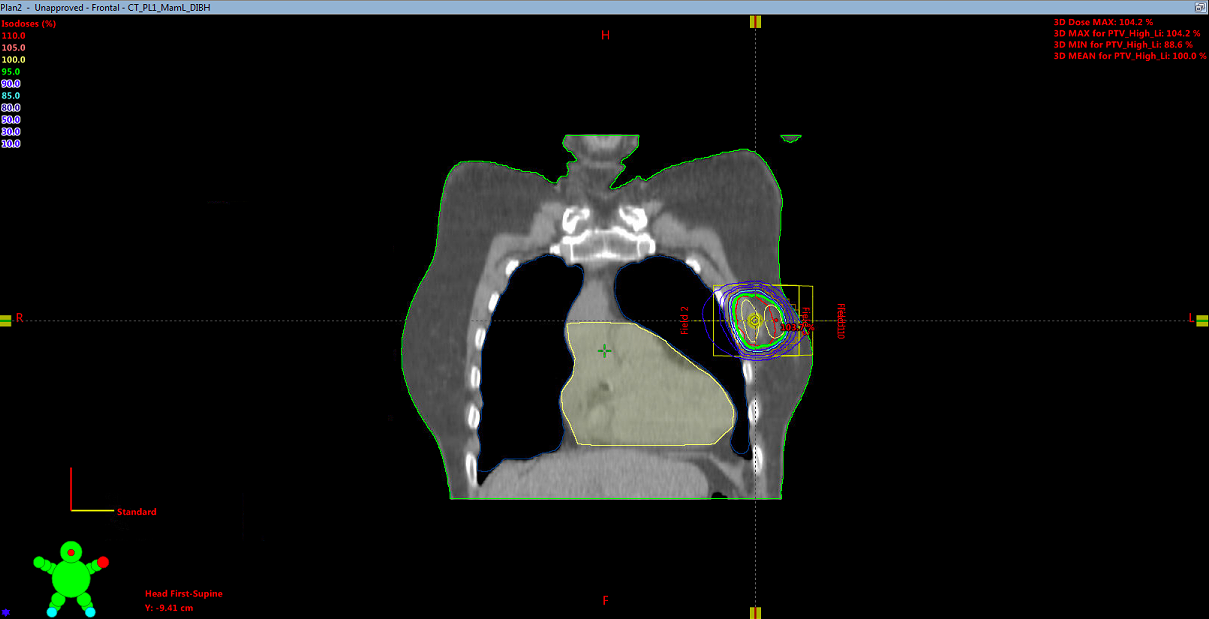
\includegraphics[width=\textwidth]{Bilder/Mamma2_Y.png}
  \caption{Darstellung der Dosisverteilung im Thorax in Frontalansicht.}
  \label{abb:Y2}
\end{figure}

\begin{figure}[H]
  \centering
  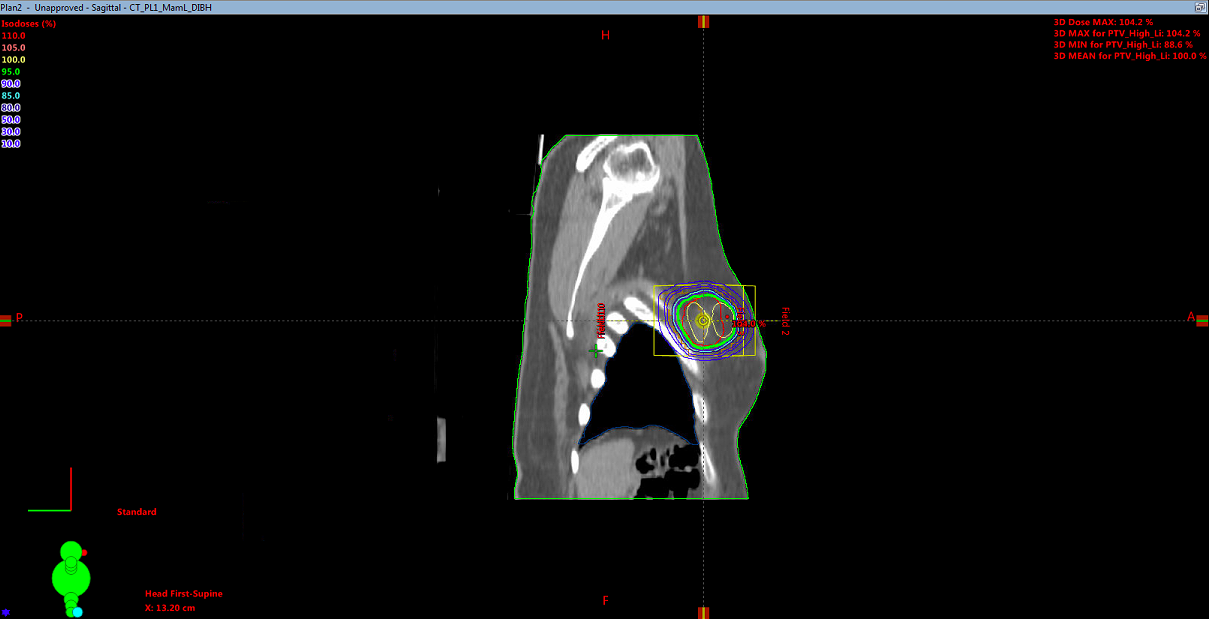
\includegraphics[width=\textwidth]{Bilder/Mamma2_X.png}
  \caption{Darstellung der Dosisverteilung im Thorax in Sagittalansicht.}
  \label{abb:X2}
\end{figure}

Auch für diesen Bestrahlungsplan wird ein DVH erzeugt, was in der Abbildung \ref{abb:DVH2}
gezeigt ist. Anhand der DVH Kurve für das PTV2 (rot) ist zu erkennen, dass in etwa $98\%$
des Volumens eine relative Dosis von $95\%$ appliziert wird. Da alle anderen DVH Kurven, außer die für das CTV2,
sehr schnell abfallen, kann geschlossen werden, dass die Risikoorgane und andere Strukturen bei
diesem Bestrahlungsplan hinreichend gut geschont werden.

\begin{figure}[H]
  \centering
  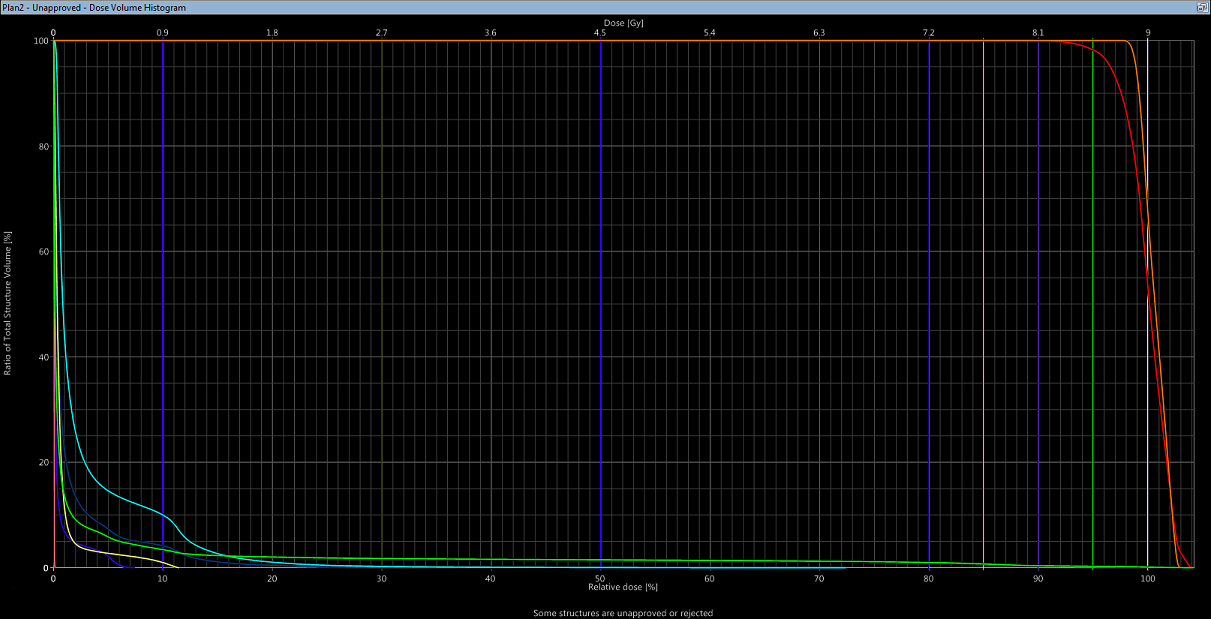
\includegraphics[width=\textwidth]{Bilder/DVH2.png}
  \caption{Dosis-Volumen-Histogramm für das PTV2 in rot und den gesamten Thorax in grün. Außerdem ist das DVH für das Herz in gelb, für die linke Lunge in hellblau, für die rechte Lunge in blau, für die gesamte Lunge in dunkelblau, für die rechte Mamma in pink und für das CTV2 in orange dargestellt.}
  \label{abb:DVH2}
\end{figure}


\subsubsection*{Summe der Bestrahlungspläne}

In der Abbildung \ref{abb:DVHsum} ist das DVH für die Summe der beiden Bestrahlungspläne
gezeigt. Bei den zwei Bestrahlungsserien wird eine gesamte Dosis von $\SI{59,4}{\gray}$ appliziert.
Anhand des DVHs kann nun überprüft werden ob die Organdosisgrenzwerte für die Lunge und für
das Herz eingehalten worden sind. In der gesamten Lunge darf die mittlere Dosis $\SI{20}{\gray}$ nicht
überschreiten und weniger als $30\%$ des Volumens der Lunge darf eine Dosis von $\SI{20}{\gray}$ erhalten \cite{grenz}.
Bei dieser Bestrahlung erhält die gesamte Lunge eine mittlere Dosis von $\SI{2,944}{\gray}$ und etwa $5\%$ des Volumens
erhält eine Dosis von $\SI{20}{\gray}$.
Der Grenzwert wird auch eingehalten, wenn die Lungenflügel getrennt betrachtet werden.
Die mittlere Dosis des rechten Lungenflügels beträgt $\SI{0.061}{\gray}$ und des linken Lungenflügels $\SI{6.982}{\gray}$.
Bei dem rechten Lungenflügel beträgt die maximale Dosis $\SI{0.972}{\gray}$, deshalb muss dort die Volumendosis nicht betrachtet werden.
Bei dem linken Lungenflügel wird in etwa $12\%$ des Volumens eine Dosis von $\SI{20}{\gray}$ deponiert.
Bei dem Herzen darf die mittlere Dosis $\SI{26}{\gray}$ nicht überschreiten
und weniger als $46\%$ des Volumens darf eine Dosis von $\SI{30}{\gray}$ erhalten \cite{grenz}.
Bei dieser Bestrahlung erhält das Herz eine mittlere Dosis von $\SI{2,263}{\gray}$ und etwa $2\%$ des Volumens
erhält eine Dosis von $\SI{30}{\gray}$. Die Organdosisgrenzwerte sind also nicht überschritten worden.

\begin{figure}[H]
  \centering
  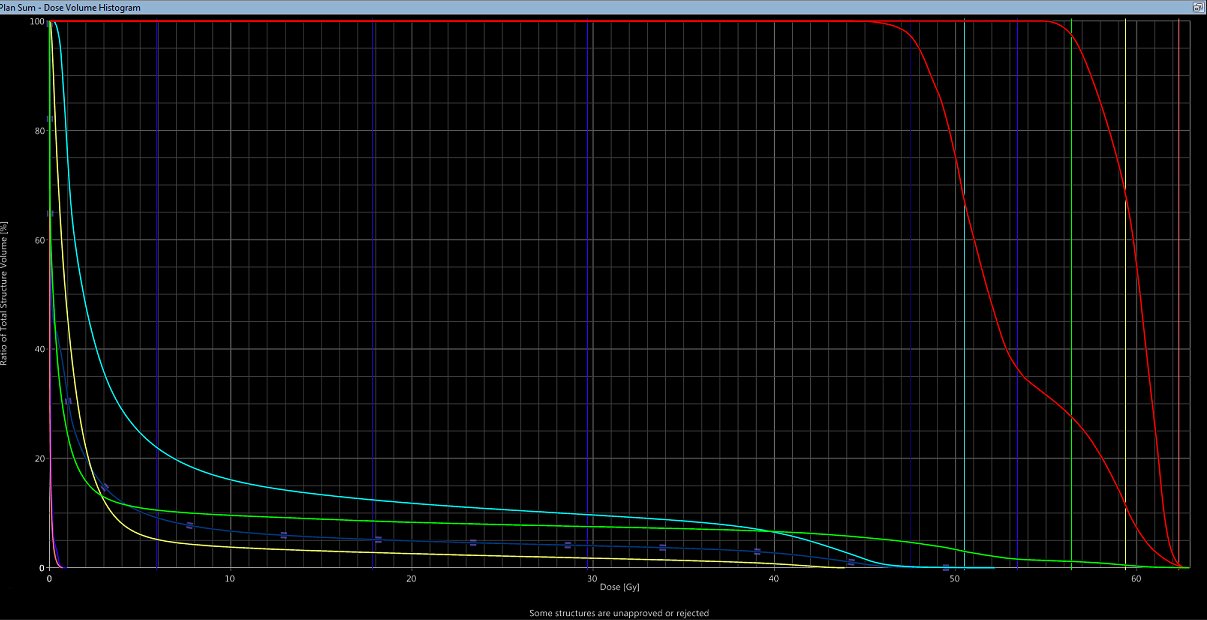
\includegraphics[width=\textwidth]{Bilder/DVHsumme.png}
  \caption{Dosis-Volumen-Histogramm für die Summe der beiden Pläne. Das DVH für die beiden PTVs in rot und den gesamten Thorax in grün. Außerdem ist das DVH für das Herz in gelb, für die linke Lunge in hellblau, für die rechte Lunge in blau, für die gesamte Lunge in dunkelblau und für die rechte Mamma in pink.}
  \label{abb:DVHsum}
\end{figure}

Mit den gewählten Feldern für die beiden Bestrahlungsserien konnte in beiden Fällen
das PTV nicht komplett mit der $95\%$ Isodosenlinie umschlossen werden. Da in beiden
Fällen nur ein kleiner Teil des Zielvolumens eine geringere Dosis als $95\%$ erhält und
die Dosiswerte für die Lunge und das Herz weit unterhalb der Grenzwerte liegen, sind die
erstellten Pläne gut für diese Strahlentherapie geeignet.
